\section{An aside: Quaternions}

Complex numbers extend the real numbers by adjoining a new unit $i$ with $i^2=-1$.  Quaternions extend the complex numbers further by adjoining \emph{three} imaginary units.

Quaternions were introduced by the Irish mathematician William Rowan Hamilton in 1843 as a way to extend complex numbers to describe rotations in three dimensions. After years of trying (and failing) to build a consistent “three–dimensional complex arithmetic”, Hamilton realised that the key was to move to four components and to accept that multiplication need not commute. On 16th October 1843, while walking in Dublin, he famously carved the fundamental relations 
\begin{equation*}
\mathbf{i}^2=\mathbf{j}^2=\mathbf{k}^2=\mathbf{i}\mathbf{j}\mathbf{k}=-1.
\end{equation*}
into the stone of Brougham Bridge. 
\begin{center}
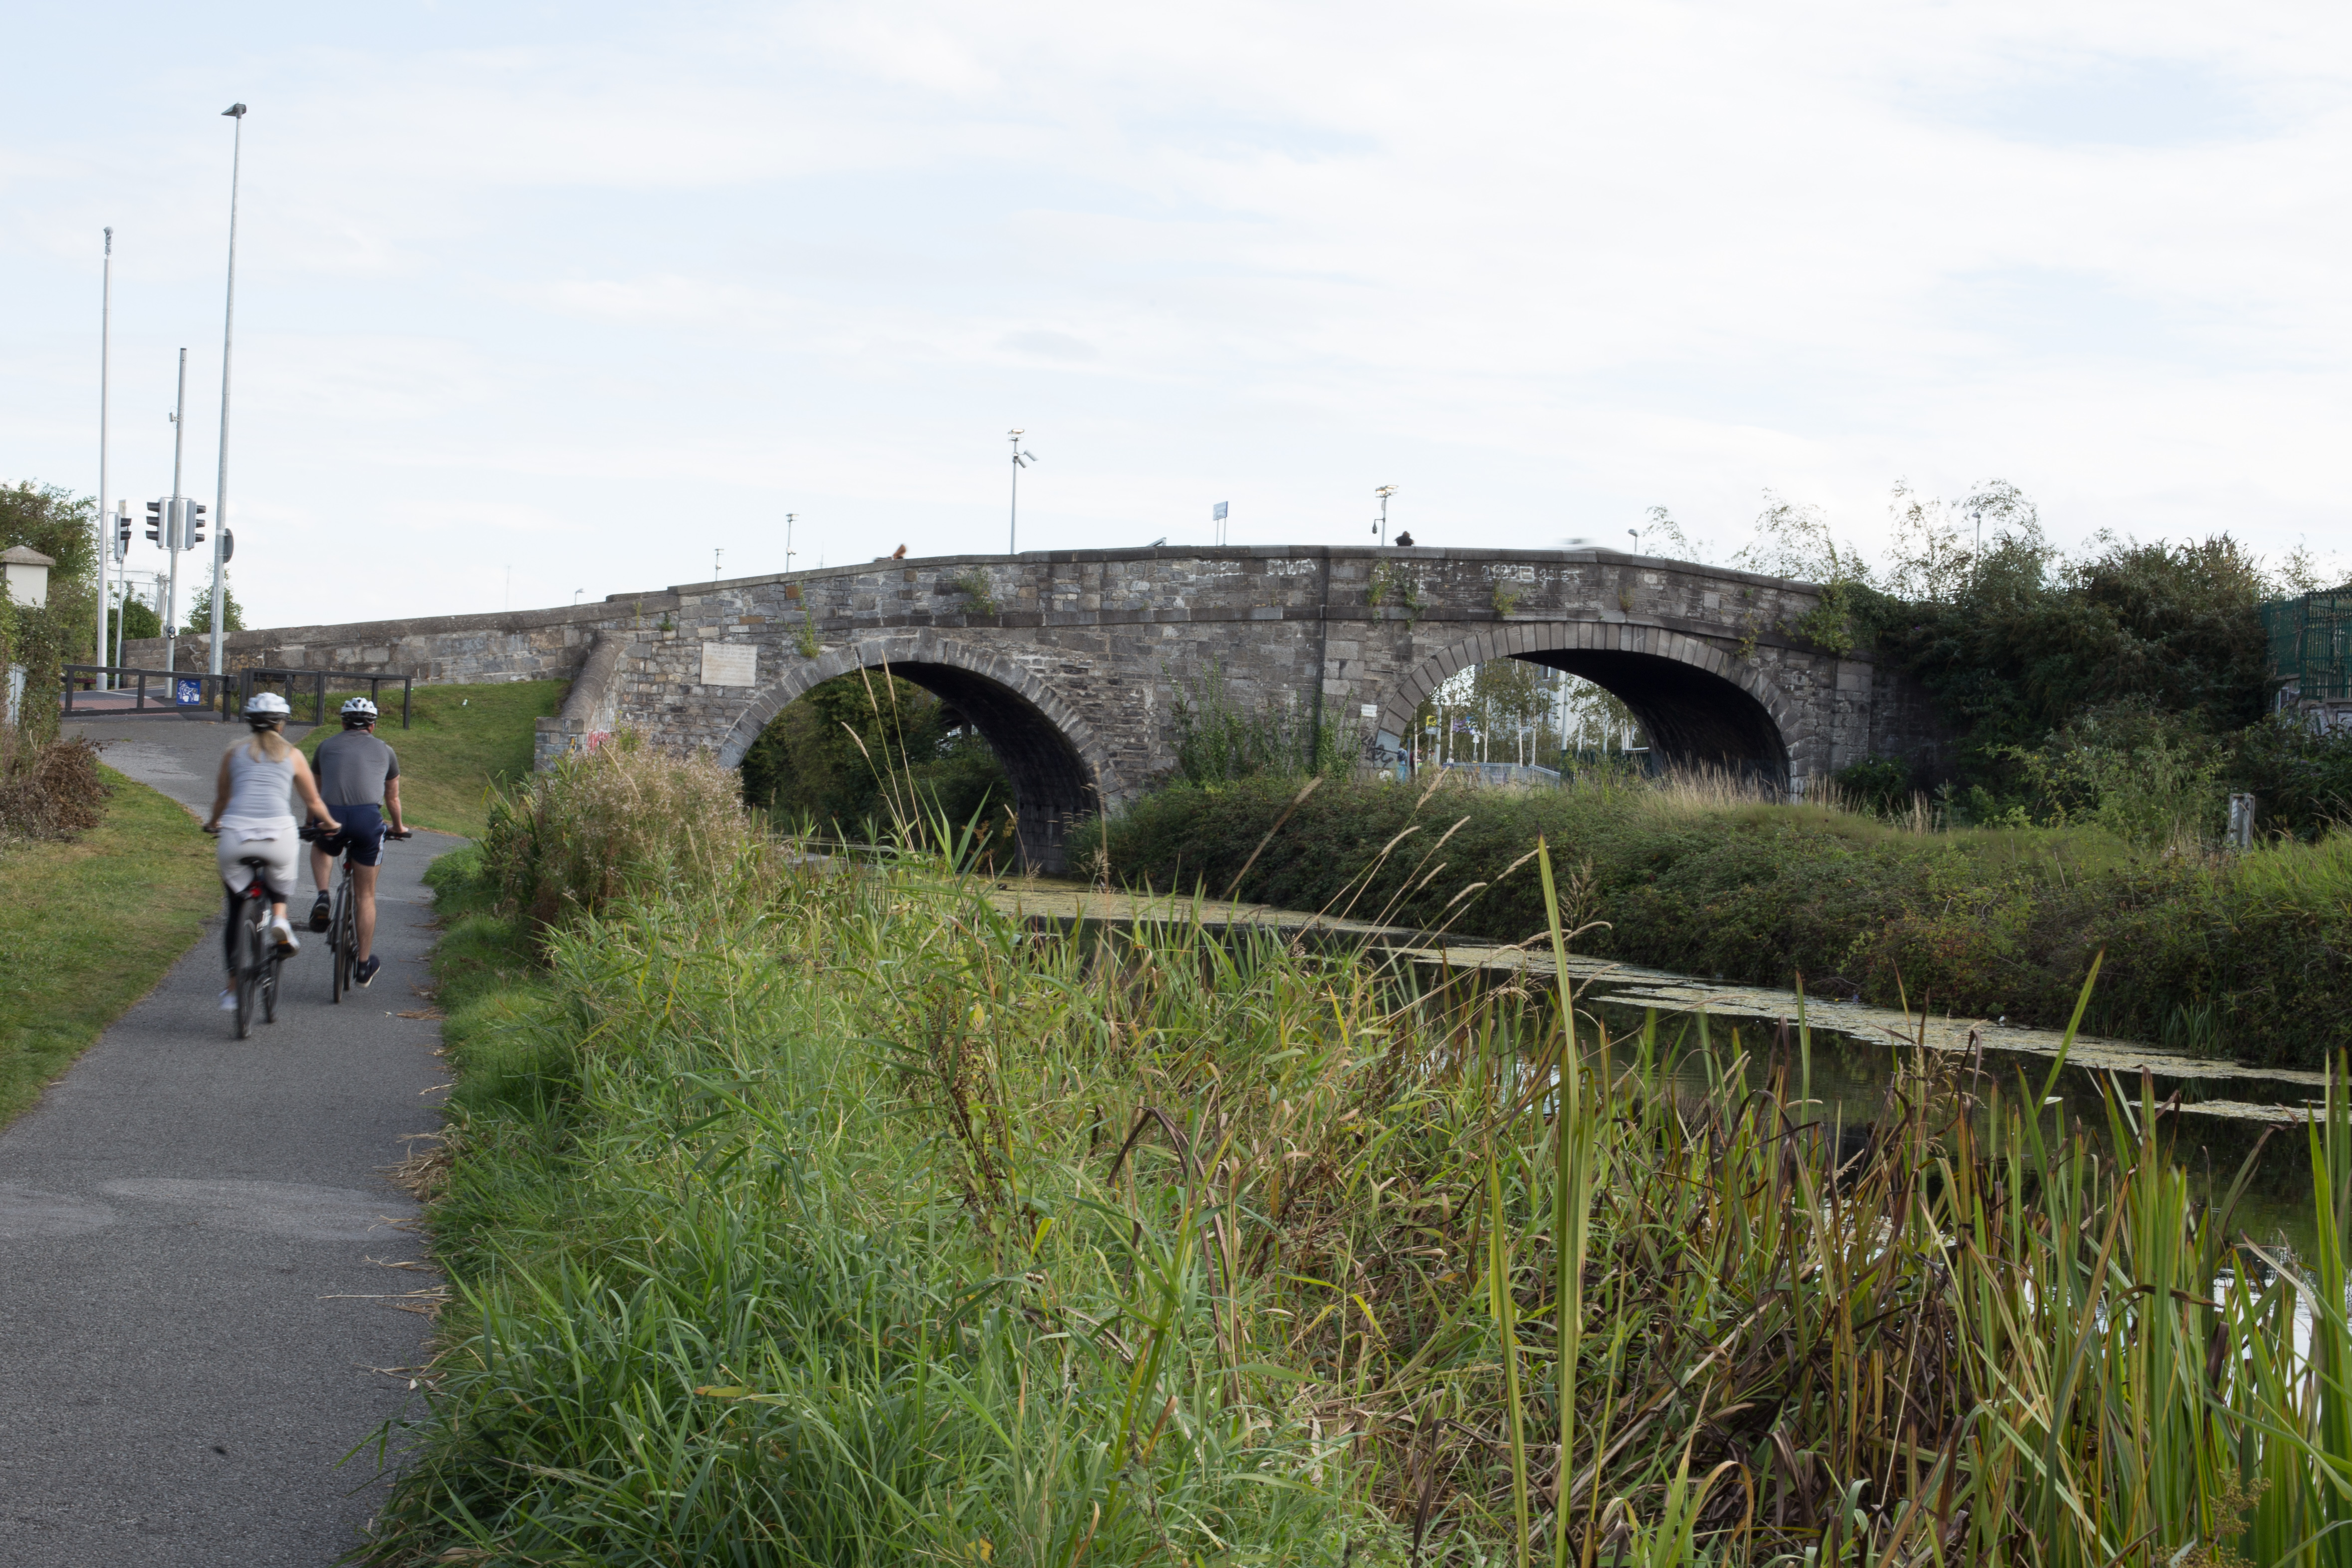
\includegraphics[width=0.5\textwidth]{Broom_Bridge.jpg}
\end{center}

Quaternions quickly attracted attention in 19th-century mathematical physics and geometry, but they were later overshadowed in many applications by the vector calculus of Gibbs and Heaviside. In the late 20th century they saw a major revival in engineering and computing—especially in robotics, aerospace, and computer graphics—because unit quaternions provide a numerically stable and efficient way to represent 3D rotations without the singularities that can occur with Euler angles, which appear when using vectors.

\subsection{Definitions and Arithmetic}

\begin{df}{Quaternion}
A \emph{quaternion} is an expression of the form
\begin{equation*}
q = a + b\,\mathbf{i} + c\,\mathbf{j} + d\,\mathbf{k}
\end{equation*}
where $a,b,c,d\in\R$ and the symbols $\mathbf{i},\mathbf{j},\mathbf{k}$ satisfy
\begin{equation*}
\mathbf{i}^2=\mathbf{j}^2=\mathbf{k}^2=\mathbf{i}\mathbf{j}\mathbf{k}=-1.
\end{equation*}
The set of all quaternions is denoted $\mathbb H$.
\end{df}

From the defining relations one can derive the multiplication rules
\begin{center}
\renewcommand{\arraystretch}{1.2}
\begin{tabular}{c|ccc}
$\cdot$ & $\mathbf{i}$ & $\mathbf{j}$ & $\mathbf{k}$\\
\hline
$\mathbf{i}$ & $-1$ & $\mathbf{k}$ & $-\mathbf{j}$\\
$\mathbf{j}$ & $-\mathbf{k}$ & $-1$ & $\mathbf{i}$\\
$\mathbf{k}$ & $\mathbf{j}$ & $-\mathbf{i}$ & $-1$\\
\end{tabular}
\end{center}

\caution Quaternion multiplication is \emph{not commutative}. For example,
\begin{equation*}
\mathbf{i}\mathbf{j}=\mathbf{k}\qquad\text{but}\qquad \mathbf{j}\mathbf{i}=-\mathbf{k}.
\end{equation*}

\begin{df}{Scalar and vector parts}
Write a quaternion as
\begin{equation*}
q = a + \vec v,\qquad \text{where}\quad \vec v=b\,\mathbf{i}+c\,\mathbf{j}+d\,\mathbf{k}.
\end{equation*}
We call $a$ the \emph{scalar part} of $q$ and $\vec v$ the \emph{vector part}.
\end{df}

Addition and subtraction are componentwise (exactly as for complex numbers):
\begin{equation*}
(a,\,b,\,c,\,d)\pm (e,\,f,\,g,\,h)=(a\pm e,\,b\pm f,\,c\pm g,\,d\pm h).
\end{equation*}
Multiplication is defined using distributivity together with the table above.

\begin{example}
Compute $(1+\mathbf{i})(1+\mathbf{j})$.
\begin{align*}
(1+\mathbf{i})(1+\mathbf{j})&=1+\mathbf{j}+\mathbf{i}+\mathbf{i}\mathbf{j}\\
&=1+\mathbf{i}+\mathbf{j}+\mathbf{k}.
\end{align*}
If we swap the factors,
\begin{align*}
(1+\mathbf{j})(1+\mathbf{i})&=1+\mathbf{i}+\mathbf{j}+\mathbf{j}\mathbf{i}\\
&=1+\mathbf{i}+\mathbf{j}-\mathbf{k},
\end{align*}
so the order matters.
\end{example}

\subsection{Conjugate, Norm and Inverse}

Quaternions have an analogue of complex conjugation.

\begin{df}{Quaternion conjugate}
For $q=a+b\mathbf{i}+c\mathbf{j}+d\mathbf{k}$, the \emph{conjugate} is
\begin{equation*}
\conj{q}=a-b\mathbf{i}-c\mathbf{j}-d\mathbf{k}.
\end{equation*}
\end{df}

\begin{df}{Norm}
The \emph{norm} of $q$ is defined by
\begin{equation*}
\lVert q\rVert = \sqrt{q\conj{q}}=\sqrt{a^2+b^2+c^2+d^2}.
\end{equation*}
\end{df}

\begin{example}
Let $q=2-\mathbf{i}+2\mathbf{j}+\mathbf{k}$. Then
\begin{align*}
\conj{q}&=2+\mathbf{i}-2\mathbf{j}-\mathbf{k},\\
\lVert q\rVert&=\sqrt{2^2+(-1)^2+2^2+1^2}=\sqrt{10}.
\end{align*}
\end{example}

Just like complex numbers, the norm is useful for division.

\begin{thm}{Inverse of a nonzero quaternion}
If $q\neq 0$, then $q$ has a multiplicative inverse
\begin{equation*}
q^{-1}=\frac{\conj{q}}{\lVert q\rVert^2}.
\end{equation*}
\end{thm}

\begin{example}
Find the inverse of $q=1+\mathbf{i}+\mathbf{j}+\mathbf{k}$.
\begin{align*}
\conj{q}&=1-\mathbf{i}-\mathbf{j}-\mathbf{k},\\
\lVert q\rVert^2&=1^2+1^2+1^2+1^2=4,\\
q^{-1}&=\frac{1}{4}\,(1-\mathbf{i}-\mathbf{j}-\mathbf{k}).
\end{align*}
\end{example}

\caution Because multiplication is not commutative, one must distinguish between left and right division in more advanced settings. In this course we will only divide by placing the inverse on the \emph{right}: $\,p/q:=p\,q^{-1}$.

\subsection{Unit Quaternions and 3D Rotations}

A key application of quaternions is the description of rotations in $\R^3$.

\begin{df}{Pure imaginary quaternion}
A quaternion with zero scalar part,
\begin{equation*}
\vec v=b\mathbf{i}+c\mathbf{j}+d\mathbf{k},
\end{equation*}
is called \emph{pure imaginary}.  We identify it with the vector $(b,c,d)\in\R^3$.
\end{df}

\begin{df}{Unit quaternion}
A quaternion $q$ with $\lVert q\rVert=1$ is called a \emph{unit quaternion}.
\end{df}

Any rotation by angle $\theta$ about a unit axis $\hat n\in\R^3$ can be encoded by the unit quaternion
\begin{equation*}
q = \cos\frac{\theta}{2} + \sin\frac{\theta}{2}\,(n_1\mathbf{i}+n_2\mathbf{j}+n_3\mathbf{k}),\qquad \hat n=(n_1,n_2,n_3),\ \lVert\hat n\rVert=1.
\end{equation*}
Given a vector $\vec v\in\R^3$ (viewed as a pure imaginary quaternion), the rotated vector is
\begin{equation*}
\vec v\,' = q\,\vec v\,q^{-1}.
\end{equation*}

\begin{example}
Rotate $(1,0,0)$ by $90^\circ$ about the $z$--axis.

The axis is $\hat n=(0,0,1)$ and $\theta=\pi/2$, so
\begin{equation*}
q=\cos\frac{\pi}{4}+\sin\frac{\pi}{4}\,\mathbf{k}=\frac{\sqrt 2}{2}+\frac{\sqrt 2}{2}\,\mathbf{k},\qquad q^{-1}=\conj{q}=\frac{\sqrt 2}{2}-\frac{\sqrt 2}{2}\,\mathbf{k}.
\end{equation*}
Let $\vec v=\mathbf{i}$ (since $(1,0,0)$ corresponds to $\mathbf{i}$). Then
\begin{align*}
\vec v\,' &= q\,\mathbf{i}\,q^{-1}
=\left(\tfrac{\sqrt2}{2}+\tfrac{\sqrt2}{2}\mathbf{k}\right)\mathbf{i}\left(\tfrac{\sqrt2}{2}-\tfrac{\sqrt2}{2}\mathbf{k}\right)\\
&=\left(\tfrac{\sqrt2}{2}\mathbf{i}+\tfrac{\sqrt2}{2}\mathbf{k}\mathbf{i}\right)\left(\tfrac{\sqrt2}{2}-\tfrac{\sqrt2}{2}\mathbf{k}\right)
=\left(\tfrac{\sqrt2}{2}\mathbf{i}+\tfrac{\sqrt2}{2}\mathbf{j}\right)\left(\tfrac{\sqrt2}{2}-\tfrac{\sqrt2}{2}\mathbf{k}\right)\\
&= \mathbf{j}.
\end{align*}
Thus $(1,0,0)$ rotates to $(0,1,0)$, as expected.
\end{example}

\secbreak

\begin{exercise}{}
Use the multiplication table to compute $\mathbf{i}\mathbf{k}$ and $\mathbf{k}\mathbf{i}$. What do you notice?
\end{exercise}
\begin{solution}
From the table, $\mathbf{i}\mathbf{k}=-\mathbf{j}$ and $\mathbf{k}\mathbf{i}=\mathbf{j}$. They differ by a minus sign, illustrating non-commutativity.
\end{solution}

\begin{exercise}{}
Let $q=3-2\mathbf{i}+\mathbf{j}$. Compute $\conj{q}$, $\lVert q\rVert$, and $q^{-1}$.
\end{exercise}
\begin{solution}
We have $\conj{q}=3+2\mathbf{i}-\mathbf{j}$ and
\begin{equation*}
\lVert q\rVert=\sqrt{3^2+(-2)^2+1^2+0^2}=\sqrt{14}.
\end{equation*}
Hence
\begin{equation*}
q^{-1}=\frac{\conj{q}}{\lVert q\rVert^2}=\frac{1}{14}\,(3+2\mathbf{i}-\mathbf{j}).
\end{equation*}
\end{solution}

\begin{exercise}{}
Let $\hat n=(1,0,0)$ and $\theta=\pi$. Write down the unit quaternion $q$ describing rotation by $\pi$ about the $x$--axis, and compute $q\,\mathbf{j}\,q^{-1}$.
\end{exercise}
\begin{solution}
Here $q=\cos(\pi/2)+\sin(\pi/2)\,\mathbf{i}=\mathbf{i}$ and $q^{-1}=\conj{q}=-\mathbf{i}$.
Then
\begin{equation*}
q\,\mathbf{j}\,q^{-1}=\mathbf{i}\,\mathbf{j}\,(-\mathbf{i})=-(\mathbf{i}\mathbf{j})\mathbf{i}=-\mathbf{k}\mathbf{i}=-\mathbf{j}.
\end{equation*}
So the $y$--axis is sent to $-y$, as expected for a $180^\circ$ rotation about the $x$--axis.
\end{solution}
